\section{RemOve And Retrain}\label{section:roar}

The ROAR (RemOve And Retrain) framework \cite{hooker2018benchmark} is another approach to compare XAI methods. The assumption is that if the feature attribution is correct, then by removing those features, the classifies should degrade. This assumption is based on the work done by Samek et al.\cite{samek2016evaluating} and shows promising results. Hooker argues that the method violates the key assumption of machine learning, where the training data and the test data have to be from the same distribution. By removing attributed features, we are creating data samples that come from different distribution, and therefore loss in the classification performance might be due to the distribution shift. To solve that problem, the authors propose to retrain the model on the dataset with removed features and then compare the models' performance.

\begin{figure}[ht]
    \centering
    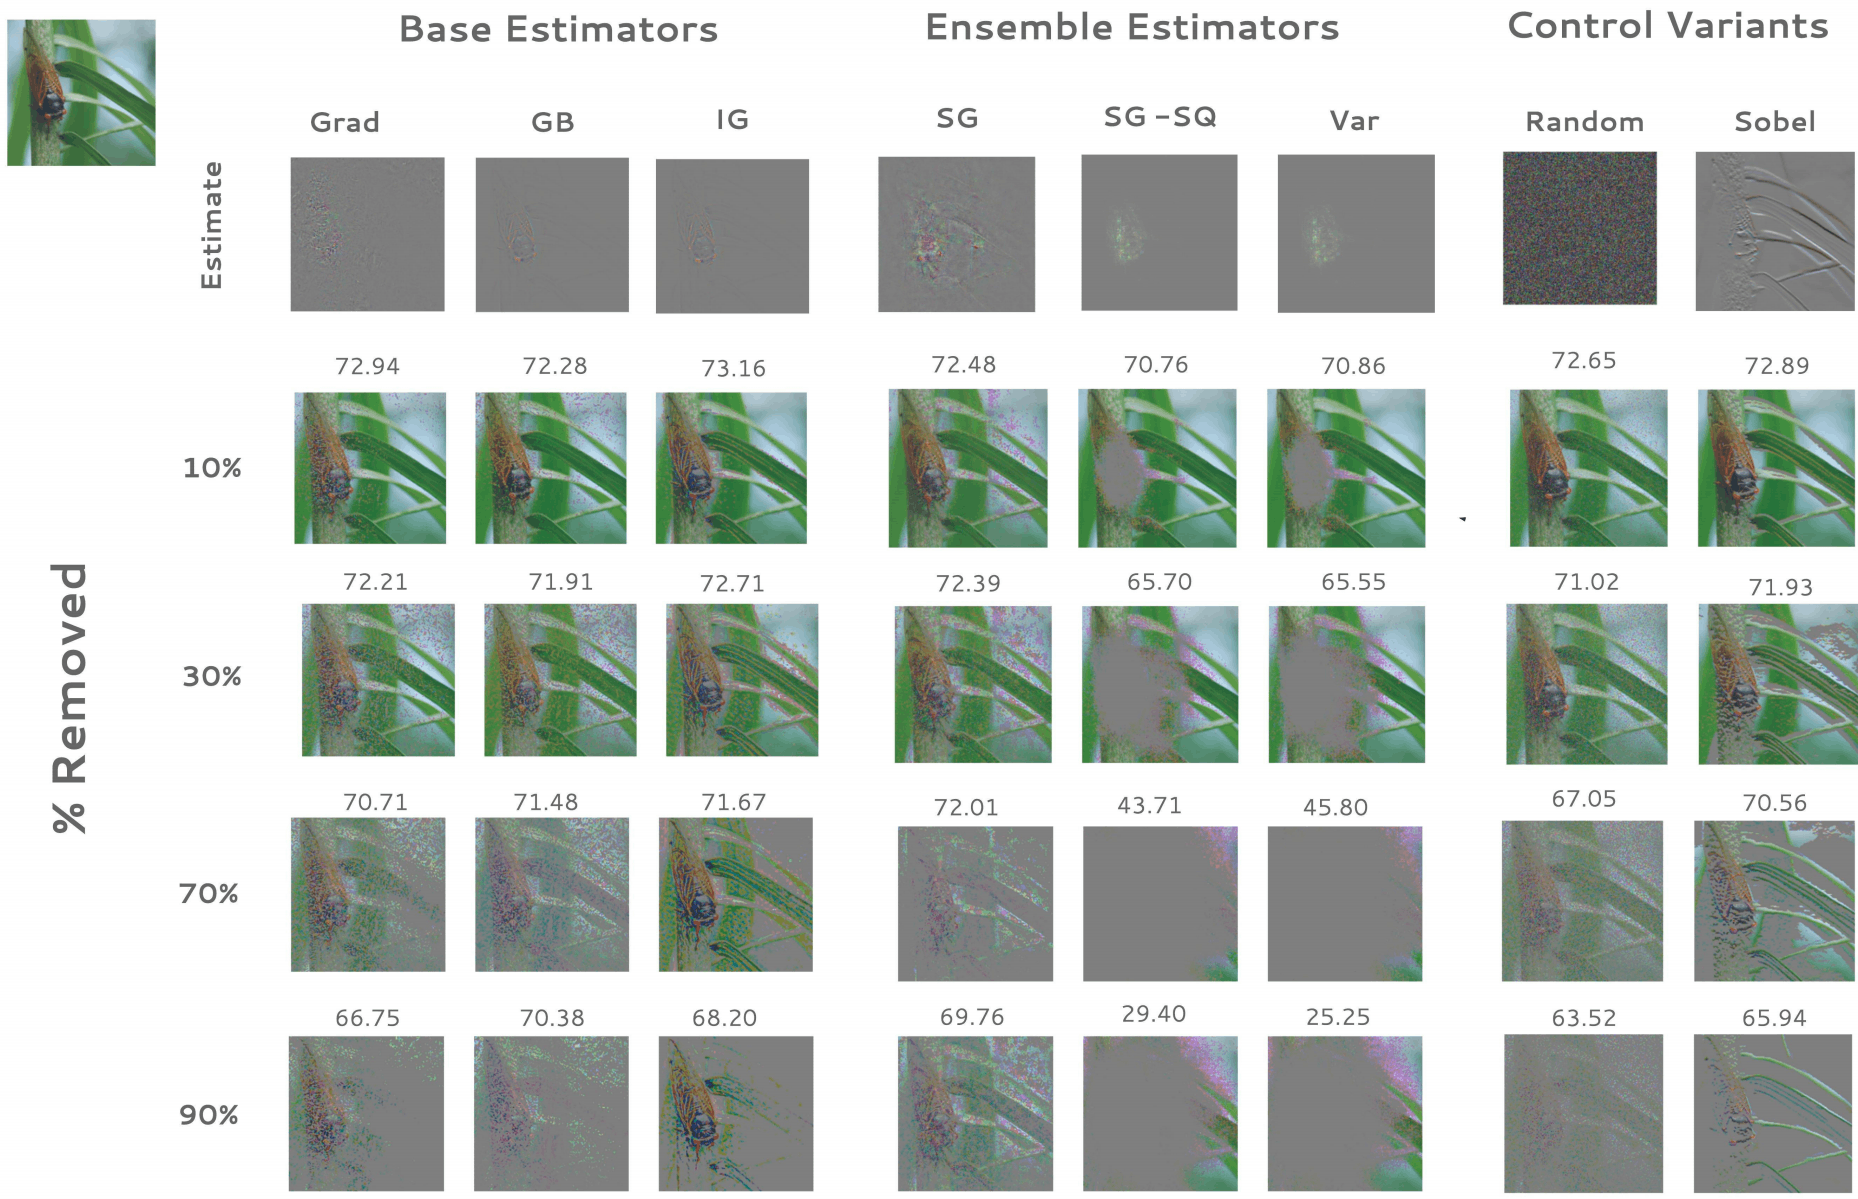
\includegraphics[width=\textwidth]{methods/images/roar-remove.png}
 \caption{Modification of the image according to the ROAR framework. The percentage of the pixels with the highest attributions is replaced by the mean value (\textit{\% Removed}). Scores above each image refer to the average test accuracy of the models trained on modified dataset. Methods used in the experiments: Saliency (GRAD) \cite{simonyan2014deep}, Guided Backpropagation (GPB) \cite{springenberg2014striving}, Integrated Gradients (IG) \cite{sundararajan2017axiomatic}, SmoothGrad (SG) and SmoothGrad-Square (SG-SQ) \cite{simonyan2014deep}, VarGrad (Var) \cite{selvaraju2017grad}, Random Bernoulli, Sobel Edge Filter. Source: \textit{A Benchmark for Interpretability Methods in Deep Neural Networks} \cite{hooker2018benchmark} }\label{fig:roar-remove}
\end{figure}

For the framework to work, it has to generate input attribution for the image and order each feature attribution from the most important to the less important. With the ordered list, it can remove a given top $t\%$ of features and replace them with a mean value of all pixels (see Fig. \ref{fig:roar-remove}). This process is repeated for $t = [0, 10, ..., 100]$ ($t$ is a percentage of all features). After removing those features, a new model is trained on the modified dataset, and the degradation in accuracy is calculated.

\begin{figure}[ht]
    \centering
    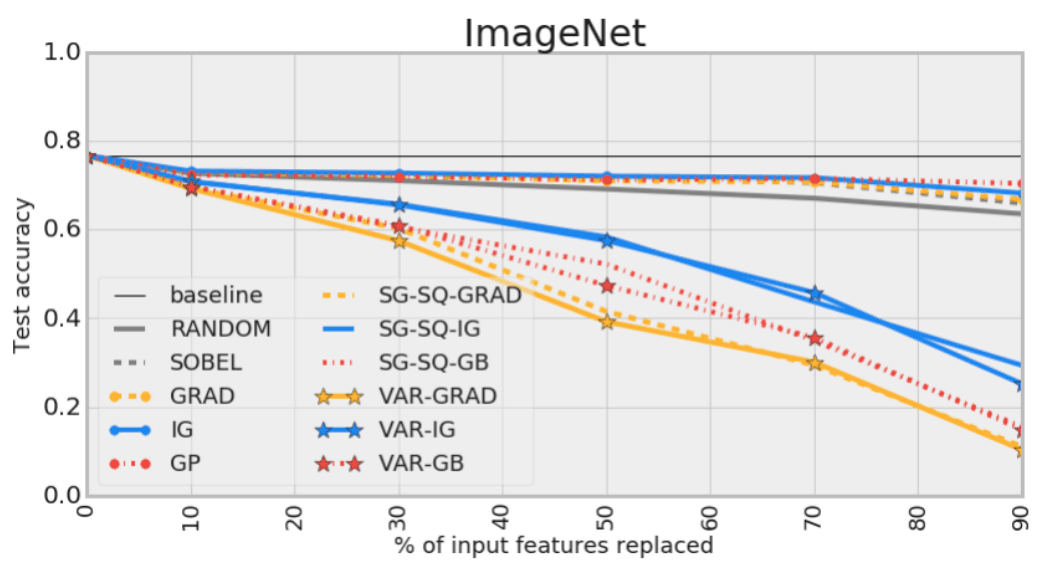
\includegraphics[width=\textwidth]{methods/images/roar-results.png}
 \caption{Results from the ROAR framework on the ImageNet dataset \cite{russakovsky2015imagenet}. A method with the highest drop (Saliency-based Noise Tunnel with VarGrad) is considered to be the one with the most relevant attribution. The biggest drop in the accuracy, the better the XAI method is according to the assumptions. Source: \textit{A Benchmark for Interpretability Methods in Deep Neural Networks} \cite{hooker2018benchmark} }\label{fig:roar-results}
\end{figure}

As shown in Figure \ref{fig:roar-results}, methods using Noise Tunnel achieve significantly better results from their original versions. The ROAR framework with its approach to compare XAI methods is an interesting proposition but has one important drawback. Every time the method is tested, we have to retrain hundreds of models, and without a computation cluster, this is not possible in an acceptable time frame.